\documentclass{beamer}
\mode<presentation> {
\usetheme{Madrid}
}
\usepackage{graphicx,caption} 
\usepackage{booktabs} 
\setbeamertemplate{caption}[numbered]

%----------------------------------------------------------------------------------------

\title[Fog-/Edge-Computing]{Fog-/Edge-Computing} 

\author{Stevan Nedic, Matthias Bögl} 
\institute[CS] 
{
Paris Lodron Universität Salzburg \\ 
\medskip
}
\date{\today } 

\begin{document}

\begin{frame}
	\titlepage 
\end{frame}

\begin{frame}
	\frametitle{Table of contents} 
	\tableofcontents 
\end{frame}

%------------------------------------------------

\section{Einführung und wichtige Begriffe} 
    \subsection{Cloud}
    \subsection{IoT}
    \subsection{Probleme}
\section{Fog/Edge Computing}
    \subsection{Was ist Fog/Edge}
    \subsection{Vor-/Nachteile}
\section{Implementierung und Herausforderungen}
    \subsection{Sicherheit und Datenschutz}
    \subsection{Netzwerk Management}
    \subsection{Technologie}
\section{Anwendung}
    \subsection{Praxis Beispiele}
    \subsection{Connected Vehicle}

%------------------------------------------------

\begin{frame}
	\begin{center}
		\Large Einführung und wichtige Begriffe
	\end{center}
\end{frame}

%------------------------------------------------

\begin{frame}
	\frametitle{\textbf{Cloud}}
	\begin{block}{\textbf{On-Demand Bereitstellung von Computer Ressourcen zur...}}
		\begin{enumerate}
			\item sofortige Saklierbarkeit im Bedarfsfall
			\item hohen Verfügbarkeit von Diensten
			\item kosteneffizienz durch Skalierbarkeit
			\item sicherheit durch Zentralisierung
		\end{enumerate}
	\end{block}
	
	\begin{block}{\textbf{auch einige Nachteile wie:}}
		\begin{enumerate}
			\item Konstante Internetverbindung benötigt
			\item Nicht real-time (Latenz)
			\item Abhängigkeit vom Dienstleister
			\item Meist nicht in geographischer Nähe
		\end{enumerate}
	\end{block}
\end{frame}

%------------------------------------------------

\begin{frame}
	\frametitle{\textbf{IoT}}
	\begin{block}{\textbf{Internet of Things}}
		\begin{enumerate}
			\item Physische Objekte mit virtueller Repräsentation
			\item Sammeln und Steuern von Daten und Geräten
			\item Kommunikation zwischen Objekten
			\item “geboren” zwischen 2008 und 2009 
		\end{enumerate}
	\end{block}
\end{frame}

%--------------------------------------

\begin{frame}
	\frametitle{\textbf{Anzahl von IoT Geräten}}
	\begin{figure}
		\includegraphics[width=\textwidth]{Iot_Geräte.png}
		\hspace*{15pt}\hbox{\scriptsize [1]\thinspace{\small\itshape statista.com}}
	\end{figure}
\end{frame}

%------------------------------------------------
\begin{frame}
	\begin{center}
		\Large Fog-/Edge- Computing
	\end{center}
\end{frame}
%------------------------------------------------%------------------------------------------------

\begin{frame}
	\frametitle{\textbf{Fog-/Edge- Computing}}
	\begin{figure}
		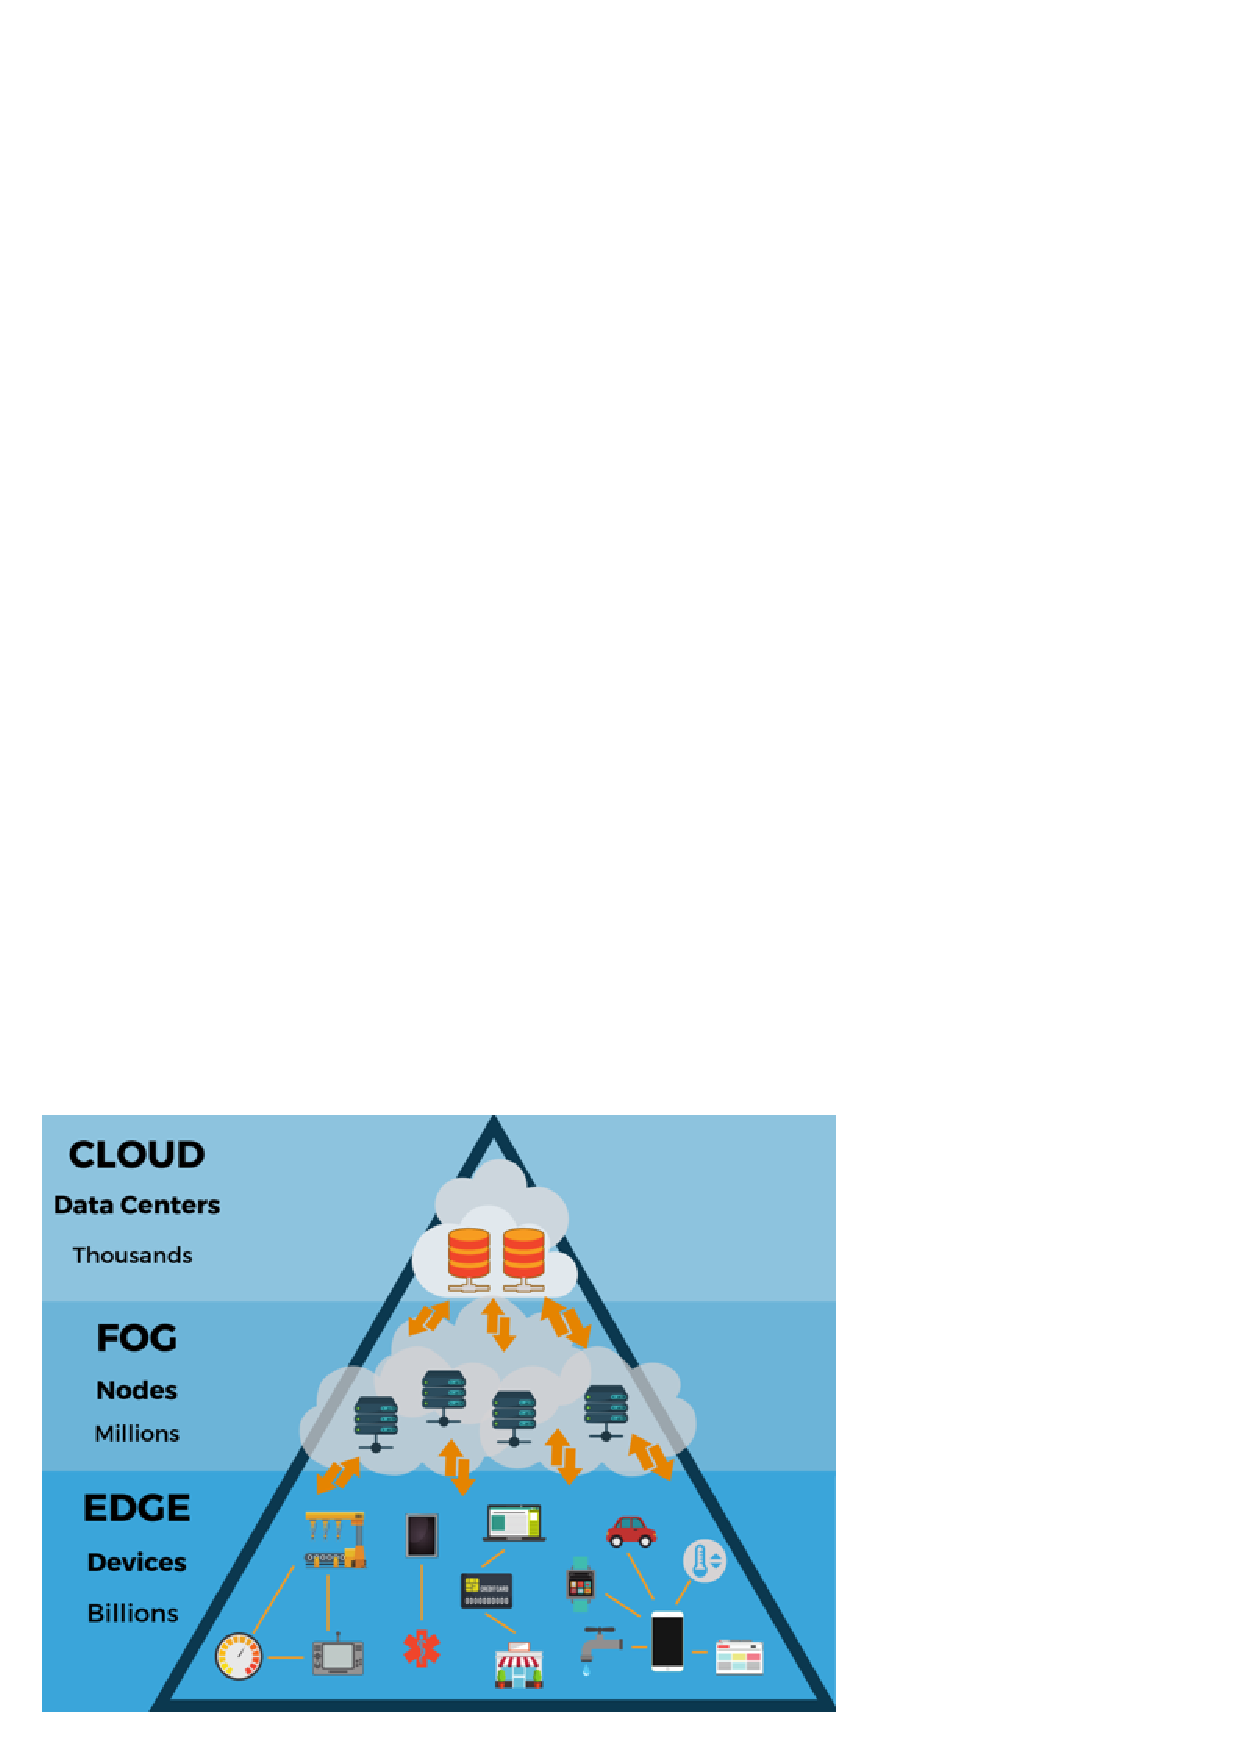
\includegraphics[scale=0.7]{Fog_Edge.png}
		\hspace*{15pt}\hbox{\scriptsize [2]\thinspace{\small\itshape thinkebiz.net}}
	\end{figure}
\end{frame}

%-----------------------------------------------

\begin{frame}
	\frametitle{\textbf{Was ist Fog-/Edge- Computing}}
	\begin{block}{\textbf{Fog-/Edge-}}
		\begin{enumerate}
			\item Erweitert Cloud Computing und ersetzt es nicht
			\item Dezentrale lokale Netzwerkarchitektur
			\item Prozesse und Ressourcen am Edge platziert
			\item Überbrückung von Cloud und Edge
		\end{enumerate}
	\end{block}
\end{frame}

%------------------------------------------------

\begin{frame}{\textbf{Vorteile/Nachteile gegenüber Cloud}}
	\begin{columns}[t] 
		
		\column{.5\textwidth} 
		\textbf{Vorteil}
		\begin{enumerate}
			\item Geringe Latenz
			\item Keine Bandbreitenprobleme
			\item Verbesserte User-Experience
			\item Power effiziente protokolle
			      (Bluetooth, ZigBee,Z-Wave)
		\end{enumerate}
		
		\column{.5\textwidth} 
		\textbf{Nachteil}
		\begin{enumerate}
			\item Komplizierteres System
			\item Größerer Kostenaufwand 
			\item VSchlechtere Skalierbarkeit 
		\end{enumerate}
	\end{columns}
\end{frame}

%-----------------------------------------------

\begin{frame}
	\Large{\centerline{Implementierung und Herausforderungen}}
\end{frame}

%----------------------------------------------------------------------------------------

\begin{frame}
	\frametitle{\textbf{Sicherheit und Datenschutz}}
	\begin{block}{\textbf{zusätzliche Schicht bietet neue Angriffsvektoren}}
		\begin{enumerate}
			\item betrügerische Fog Nodes
			\item Netzwerksicherheit
			\item Sichere und private Datenverarbeitung
			\item Einbruchserkennung
		\end{enumerate}
	\end{block}
\end{frame}

%----------------------------------------------------------------------

\begin{frame}
	\frametitle{\textbf{Netzwerk Management}}
	\begin{block}{\textbf{sehr hohe Komplexität und Anforderungen}}
		\begin{enumerate}
			\item Software Defined Networking (SDN)
			\item Network Functions Virtualization (NFV)
			\item dadurch erhöht sich Komplexität jedoch weiter
			\item kleine Fehler können zum Verfehlen von Zielen führen
		\end{enumerate}
	\end{block}
\end{frame}

%-------------------------------------------------------------

\begin{frame}
	\frametitle{\textbf{Technologie}}
	\begin{figure}
		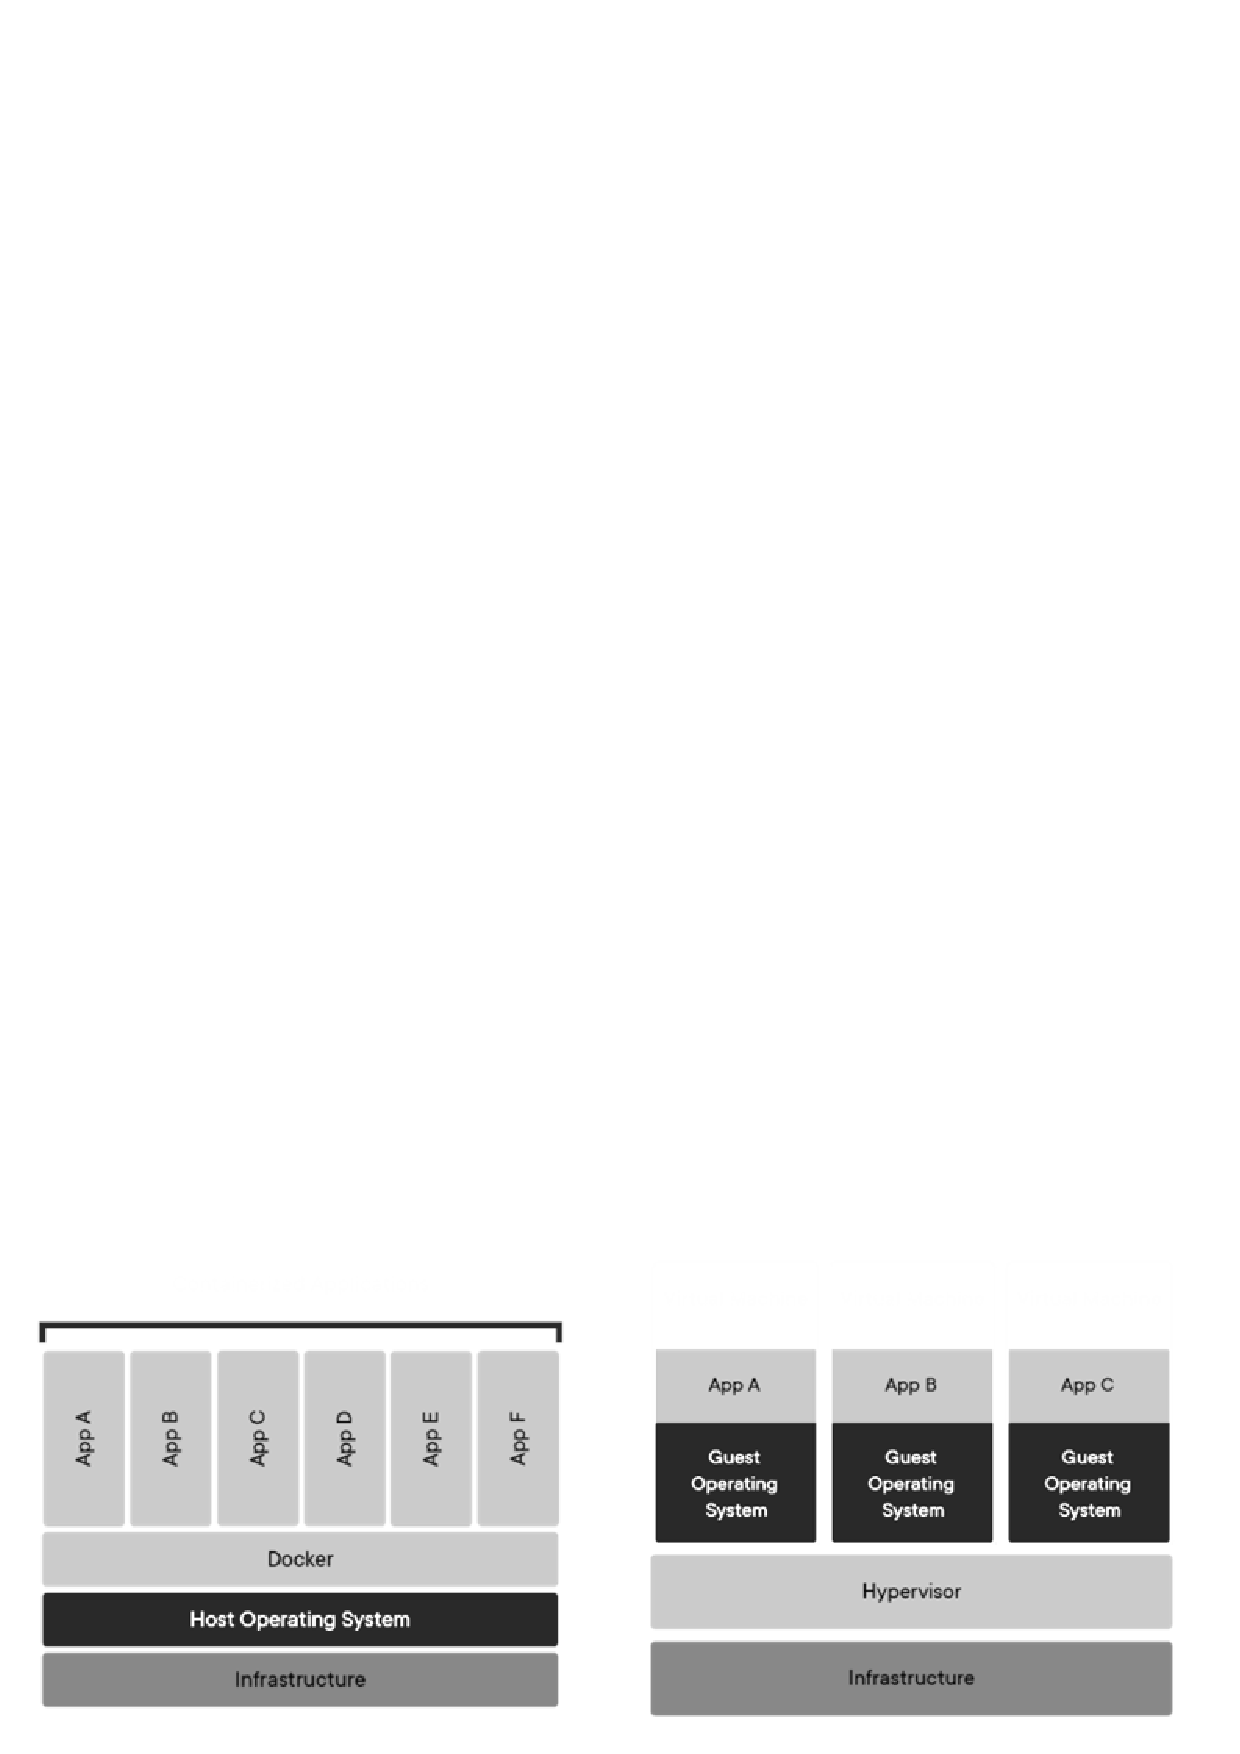
\includegraphics[width=\textwidth]{Tech.png}
		\hspace*{15pt}\hbox{\scriptsize [3]\thinspace{\small\itshape wikimedia.org}}
	\end{figure}
\end{frame}

%------------------------------------------------

\begin{frame}
	\Large{\centerline{Anwendungsgebiete}}
\end{frame}

%----------------------------------------------------------------------------------------

\begin{frame}
	\frametitle{\textbf{Praktische Beispiele}}
	\begin{columns}
		\column{0.38\linewidth}
		\centering
		\includegraphics[height=5cm, width=5cm]{Data.png}
		\hspace*{15pt}\hbox{\scriptsize [4]\thinspace{\small\itshape intel.com}}
		
		\column{0.58\linewidth}
		\begin{enumerate}
			\item Mehrere Sensoren die permanent am arbeiten sind
			\item Durchschnittlich 60 MB an Daten die analysiert und verarbeitet werden müssen 
			\item Nur mit der Cloud nicht realisierbar ohne Probleme oder Unfälle 
		\end{enumerate}
	\end{columns} 
\end{frame}

%------------------------------------------------

\begin{frame}
	\frametitle{\textbf{Connected Vehicle (CV) oder V2X}}
	\begin{figure}
		\includegraphics[width=\textwidth]{CV.png}
		\hspace*{15pt}\hbox{\scriptsize [5]\thinspace{\small\itshape thalesgroup.com}}
	\end{figure}
\end{frame}

%------------------------------------------------

\begin{frame}[allowframebreaks]
	\frametitle{\textbf{Quellen}}
	\footnotesize{
		\begin{thebibliography}{99}
			\bibitem  SSergej Svorobej, et al.
			\newblock Simulating Fog and Edge Computing Scenarios: An Overview and Research Challenges. 
			\newblock \emph MDPI, 2019. 
			
			\bibitem  SShanhe Yi, et al.
			\newblock Fog Computing: Platform and Applications. 
			\newblock \emph Third IEEE Workshop on Hot Topics in Web Systems and Technologies, 2015
			
			\bibitem  FFlavio Bonomi, et al. 
			\newblock Fog Computing and Its Role in the Internet of Things.
			\newblock \emph Cisco Systems Inc.
			
			\bibitem 1
			\newblock https://www.statista.com/statistics/1183457/iot-connected-devices-worldwide
			
			\bibitem 2
			\newblock https://www.thinkebiz.net/what-edge-computing
			
			\bibitem 3
			\newblock https://upload.wikimedia.org/wikipedia/commons/0/0a/Docker-containerized-and-vm-transparent-bg.png
			
			\bibitem 4
			\newblock https://newsroom.intel.com/editorials/krzanich-the-future-of-automated-driving/
			
			\bibitem 5
			\newblock https://www.thalesgroup.com/en/markets/digital-identity-and-security/iot/industries/automotive/use-cases/v2x
			
		\end{thebibliography}
	}
	    
\end{frame}

\end{document}